% Ablation study: Qwen and Gemma win rate, two figures side by side.
% Usage: % Ablation study: Qwen and Gemma win rate, two figures side by side.
% Usage: % Ablation study: Qwen and Gemma win rate, two figures side by side.
% Usage: % Ablation study: Qwen and Gemma win rate, two figures side by side.
% Usage: \input{docs/ablation_figure} or \input{ablation_figure} from main.tex.
% Paths assume main.tex is in repo root; else set \graphicspath{{docs/}}.
%
% Optional: \usepackage{subcaption} lets you use \subcaption{(a) Qwen-2 0.5B} etc.
% Below uses a single caption and (a)/(b) in text for maximum compatibility.

\begin{figure*}[t]
    \centering
    \begin{minipage}[t]{0.48\linewidth}
        \centering
        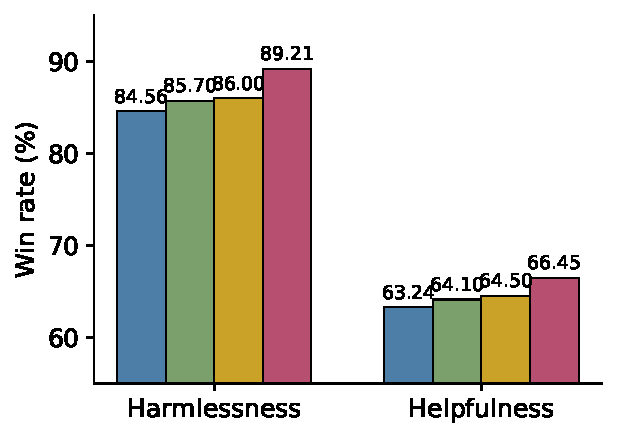
\includegraphics[width=\linewidth]{figures/ablation_winrate_combined.pdf}
        \vspace{0.3em}
        \scriptsize\textbf{(a) Qwen-2 0.5B}
    \end{minipage}\hfill
    \begin{minipage}[t]{0.48\linewidth}
        \centering
        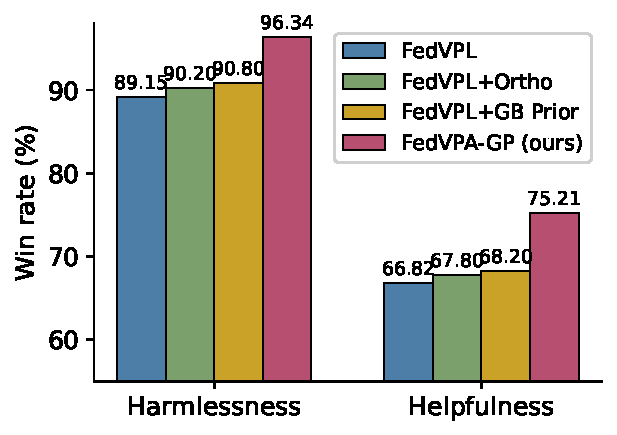
\includegraphics[width=\linewidth]{figures/ablation_winrate_combined_gemma.pdf}
        \vspace{0.3em}
        \scriptsize\textbf{(b) Gemma-2B}
    \end{minipage}
    \caption{Ablation study: helpfulness and harmlessness win rate (\%). (a) Qwen-2 0.5B. (b) Gemma-2B. Methods: FedVPL, FedVPL+Ortho, FedVPL+GB Prior, FedVPA-GP.}
    \label{fig:ablation}
\end{figure*}
 or % Ablation study: Qwen and Gemma win rate, two figures side by side.
% Usage: \input{docs/ablation_figure} or \input{ablation_figure} from main.tex.
% Paths assume main.tex is in repo root; else set \graphicspath{{docs/}}.
%
% Optional: \usepackage{subcaption} lets you use \subcaption{(a) Qwen-2 0.5B} etc.
% Below uses a single caption and (a)/(b) in text for maximum compatibility.

\begin{figure*}[t]
    \centering
    \begin{minipage}[t]{0.48\linewidth}
        \centering
        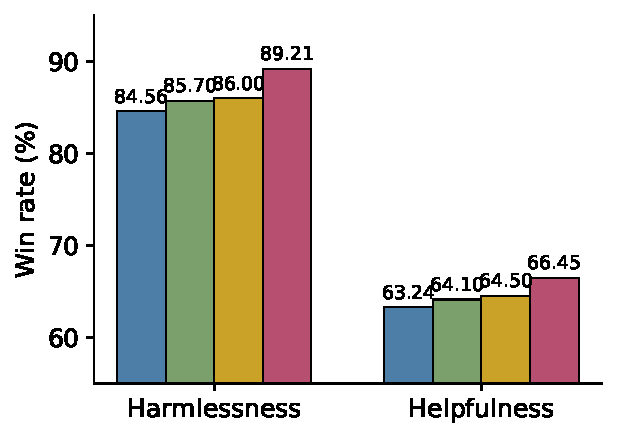
\includegraphics[width=\linewidth]{figures/ablation_winrate_combined.pdf}
        \vspace{0.3em}
        \scriptsize\textbf{(a) Qwen-2 0.5B}
    \end{minipage}\hfill
    \begin{minipage}[t]{0.48\linewidth}
        \centering
        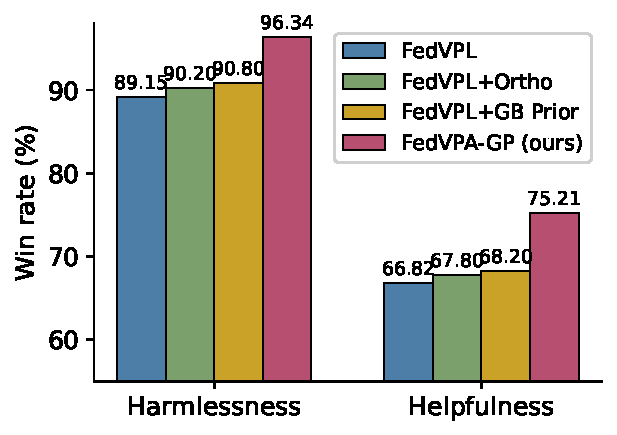
\includegraphics[width=\linewidth]{figures/ablation_winrate_combined_gemma.pdf}
        \vspace{0.3em}
        \scriptsize\textbf{(b) Gemma-2B}
    \end{minipage}
    \caption{Ablation study: helpfulness and harmlessness win rate (\%). (a) Qwen-2 0.5B. (b) Gemma-2B. Methods: FedVPL, FedVPL+Ortho, FedVPL+GB Prior, FedVPA-GP.}
    \label{fig:ablation}
\end{figure*}
 from main.tex.
% Paths assume main.tex is in repo root; else set \graphicspath{{docs/}}.
%
% Optional: \usepackage{subcaption} lets you use \subcaption{(a) Qwen-2 0.5B} etc.
% Below uses a single caption and (a)/(b) in text for maximum compatibility.

\begin{figure*}[t]
    \centering
    \begin{minipage}[t]{0.48\linewidth}
        \centering
        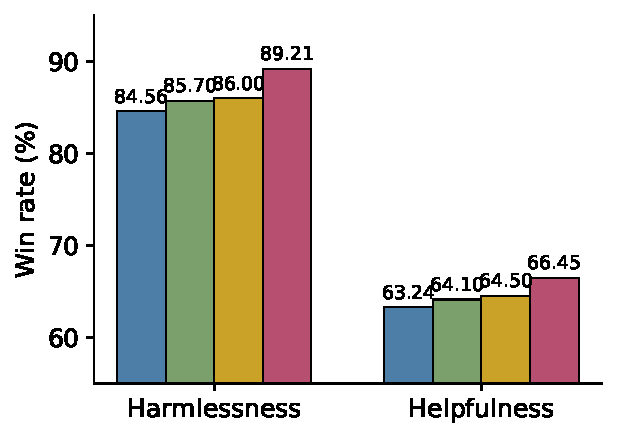
\includegraphics[width=\linewidth]{figures/ablation_winrate_combined.pdf}
        \vspace{0.3em}
        \scriptsize\textbf{(a) Qwen-2 0.5B}
    \end{minipage}\hfill
    \begin{minipage}[t]{0.48\linewidth}
        \centering
        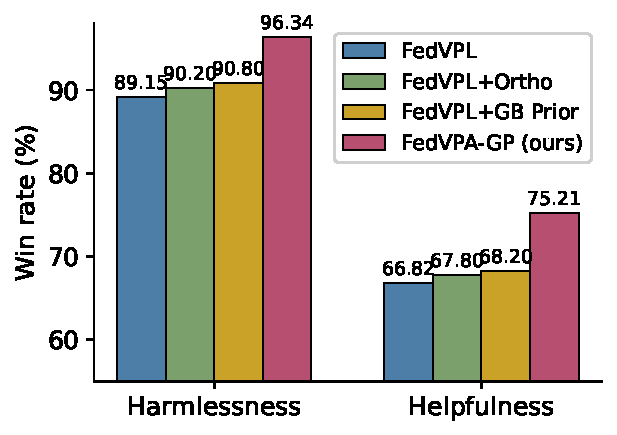
\includegraphics[width=\linewidth]{figures/ablation_winrate_combined_gemma.pdf}
        \vspace{0.3em}
        \scriptsize\textbf{(b) Gemma-2B}
    \end{minipage}
    \caption{Ablation study: helpfulness and harmlessness win rate (\%). (a) Qwen-2 0.5B. (b) Gemma-2B. Methods: FedVPL, FedVPL+Ortho, FedVPL+GB Prior, FedVPA-GP.}
    \label{fig:ablation}
\end{figure*}
 or % Ablation study: Qwen and Gemma win rate, two figures side by side.
% Usage: % Ablation study: Qwen and Gemma win rate, two figures side by side.
% Usage: \input{docs/ablation_figure} or \input{ablation_figure} from main.tex.
% Paths assume main.tex is in repo root; else set \graphicspath{{docs/}}.
%
% Optional: \usepackage{subcaption} lets you use \subcaption{(a) Qwen-2 0.5B} etc.
% Below uses a single caption and (a)/(b) in text for maximum compatibility.

\begin{figure*}[t]
    \centering
    \begin{minipage}[t]{0.48\linewidth}
        \centering
        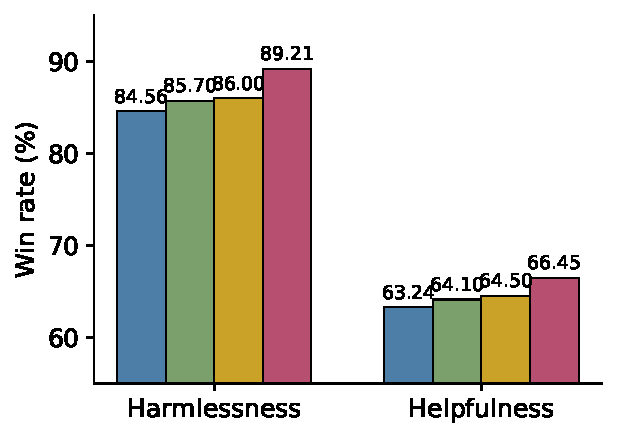
\includegraphics[width=\linewidth]{figures/ablation_winrate_combined.pdf}
        \vspace{0.3em}
        \scriptsize\textbf{(a) Qwen-2 0.5B}
    \end{minipage}\hfill
    \begin{minipage}[t]{0.48\linewidth}
        \centering
        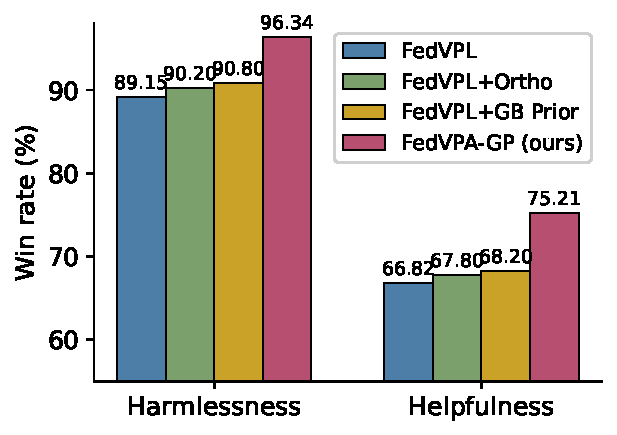
\includegraphics[width=\linewidth]{figures/ablation_winrate_combined_gemma.pdf}
        \vspace{0.3em}
        \scriptsize\textbf{(b) Gemma-2B}
    \end{minipage}
    \caption{Ablation study: helpfulness and harmlessness win rate (\%). (a) Qwen-2 0.5B. (b) Gemma-2B. Methods: FedVPL, FedVPL+Ortho, FedVPL+GB Prior, FedVPA-GP.}
    \label{fig:ablation}
\end{figure*}
 or % Ablation study: Qwen and Gemma win rate, two figures side by side.
% Usage: \input{docs/ablation_figure} or \input{ablation_figure} from main.tex.
% Paths assume main.tex is in repo root; else set \graphicspath{{docs/}}.
%
% Optional: \usepackage{subcaption} lets you use \subcaption{(a) Qwen-2 0.5B} etc.
% Below uses a single caption and (a)/(b) in text for maximum compatibility.

\begin{figure*}[t]
    \centering
    \begin{minipage}[t]{0.48\linewidth}
        \centering
        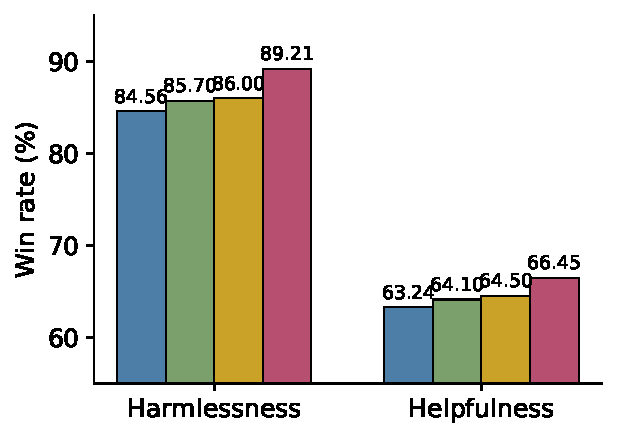
\includegraphics[width=\linewidth]{figures/ablation_winrate_combined.pdf}
        \vspace{0.3em}
        \scriptsize\textbf{(a) Qwen-2 0.5B}
    \end{minipage}\hfill
    \begin{minipage}[t]{0.48\linewidth}
        \centering
        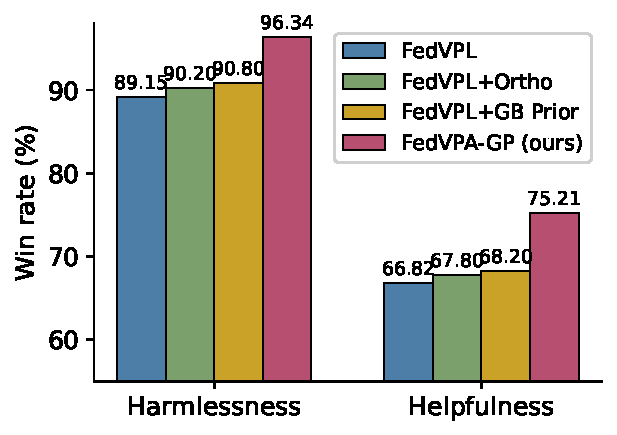
\includegraphics[width=\linewidth]{figures/ablation_winrate_combined_gemma.pdf}
        \vspace{0.3em}
        \scriptsize\textbf{(b) Gemma-2B}
    \end{minipage}
    \caption{Ablation study: helpfulness and harmlessness win rate (\%). (a) Qwen-2 0.5B. (b) Gemma-2B. Methods: FedVPL, FedVPL+Ortho, FedVPL+GB Prior, FedVPA-GP.}
    \label{fig:ablation}
\end{figure*}
 from main.tex.
% Paths assume main.tex is in repo root; else set \graphicspath{{docs/}}.
%
% Optional: \usepackage{subcaption} lets you use \subcaption{(a) Qwen-2 0.5B} etc.
% Below uses a single caption and (a)/(b) in text for maximum compatibility.

\begin{figure*}[t]
    \centering
    \begin{minipage}[t]{0.48\linewidth}
        \centering
        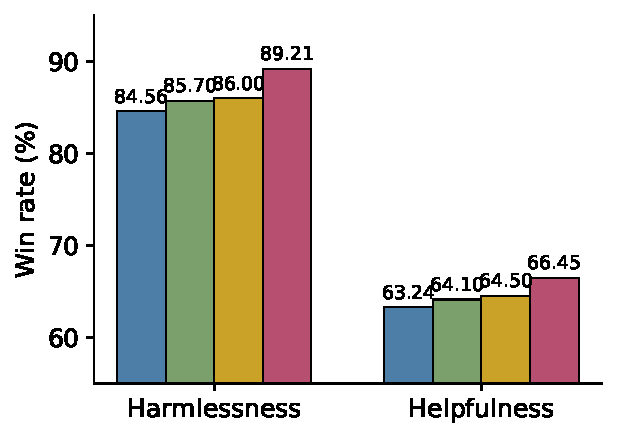
\includegraphics[width=\linewidth]{figures/ablation_winrate_combined.pdf}
        \vspace{0.3em}
        \scriptsize\textbf{(a) Qwen-2 0.5B}
    \end{minipage}\hfill
    \begin{minipage}[t]{0.48\linewidth}
        \centering
        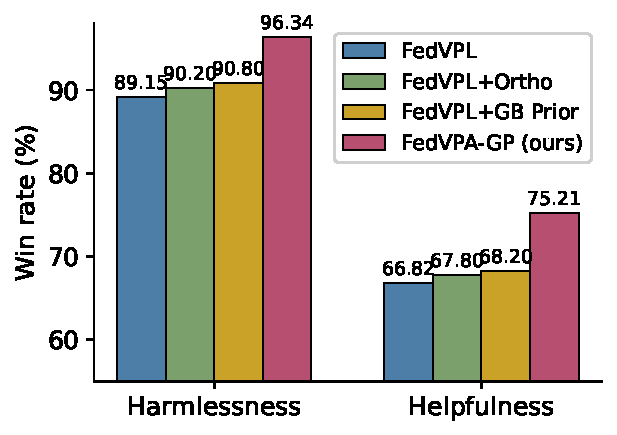
\includegraphics[width=\linewidth]{figures/ablation_winrate_combined_gemma.pdf}
        \vspace{0.3em}
        \scriptsize\textbf{(b) Gemma-2B}
    \end{minipage}
    \caption{Ablation study: helpfulness and harmlessness win rate (\%). (a) Qwen-2 0.5B. (b) Gemma-2B. Methods: FedVPL, FedVPL+Ortho, FedVPL+GB Prior, FedVPA-GP.}
    \label{fig:ablation}
\end{figure*}
 from main.tex.
% Paths assume main.tex is in repo root; else set \graphicspath{{docs/}}.
%
% Optional: \usepackage{subcaption} lets you use \subcaption{(a) Qwen-2 0.5B} etc.
% Below uses a single caption and (a)/(b) in text for maximum compatibility.

\begin{figure*}[t]
    \centering
    \begin{minipage}[t]{0.48\linewidth}
        \centering
        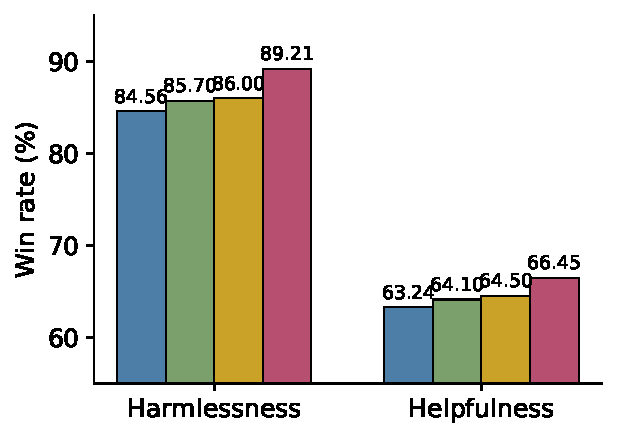
\includegraphics[width=\linewidth]{figures/ablation_winrate_combined.pdf}
        \vspace{0.3em}
        \scriptsize\textbf{(a) Qwen-2 0.5B}
    \end{minipage}\hfill
    \begin{minipage}[t]{0.48\linewidth}
        \centering
        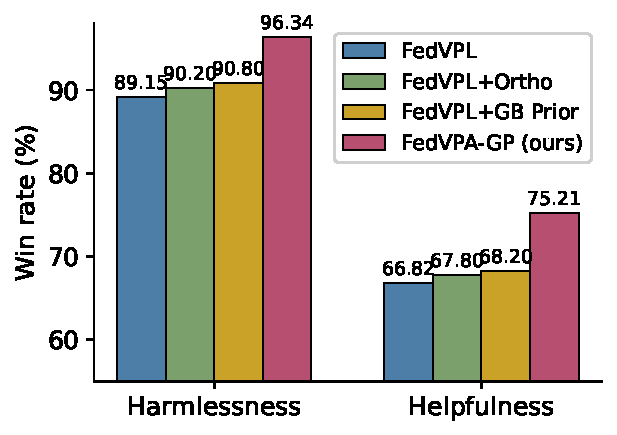
\includegraphics[width=\linewidth]{figures/ablation_winrate_combined_gemma.pdf}
        \vspace{0.3em}
        \scriptsize\textbf{(b) Gemma-2B}
    \end{minipage}
    \caption{Ablation study: helpfulness and harmlessness win rate (\%). (a) Qwen-2 0.5B. (b) Gemma-2B. Methods: FedVPL, FedVPL+Ortho, FedVPL+GB Prior, FedVPA-GP.}
    \label{fig:ablation}
\end{figure*}
 or % Ablation study: Qwen and Gemma win rate, two figures side by side.
% Usage: % Ablation study: Qwen and Gemma win rate, two figures side by side.
% Usage: % Ablation study: Qwen and Gemma win rate, two figures side by side.
% Usage: \input{docs/ablation_figure} or \input{ablation_figure} from main.tex.
% Paths assume main.tex is in repo root; else set \graphicspath{{docs/}}.
%
% Optional: \usepackage{subcaption} lets you use \subcaption{(a) Qwen-2 0.5B} etc.
% Below uses a single caption and (a)/(b) in text for maximum compatibility.

\begin{figure*}[t]
    \centering
    \begin{minipage}[t]{0.48\linewidth}
        \centering
        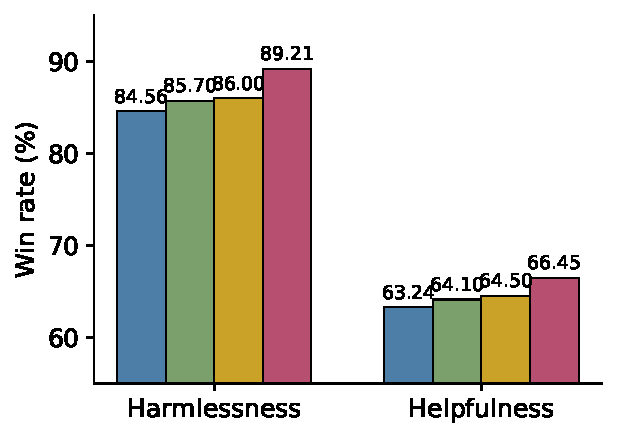
\includegraphics[width=\linewidth]{figures/ablation_winrate_combined.pdf}
        \vspace{0.3em}
        \scriptsize\textbf{(a) Qwen-2 0.5B}
    \end{minipage}\hfill
    \begin{minipage}[t]{0.48\linewidth}
        \centering
        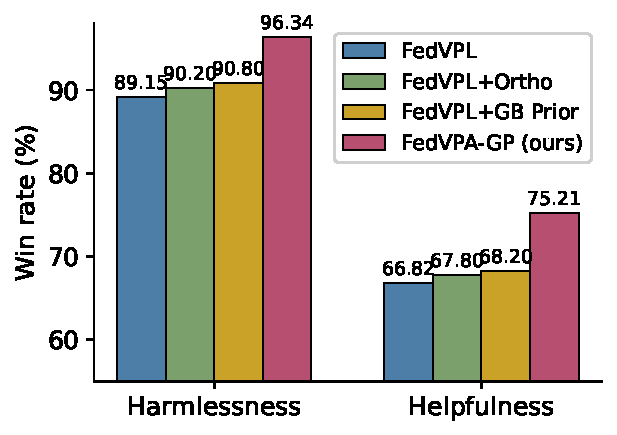
\includegraphics[width=\linewidth]{figures/ablation_winrate_combined_gemma.pdf}
        \vspace{0.3em}
        \scriptsize\textbf{(b) Gemma-2B}
    \end{minipage}
    \caption{Ablation study: helpfulness and harmlessness win rate (\%). (a) Qwen-2 0.5B. (b) Gemma-2B. Methods: FedVPL, FedVPL+Ortho, FedVPL+GB Prior, FedVPA-GP.}
    \label{fig:ablation}
\end{figure*}
 or % Ablation study: Qwen and Gemma win rate, two figures side by side.
% Usage: \input{docs/ablation_figure} or \input{ablation_figure} from main.tex.
% Paths assume main.tex is in repo root; else set \graphicspath{{docs/}}.
%
% Optional: \usepackage{subcaption} lets you use \subcaption{(a) Qwen-2 0.5B} etc.
% Below uses a single caption and (a)/(b) in text for maximum compatibility.

\begin{figure*}[t]
    \centering
    \begin{minipage}[t]{0.48\linewidth}
        \centering
        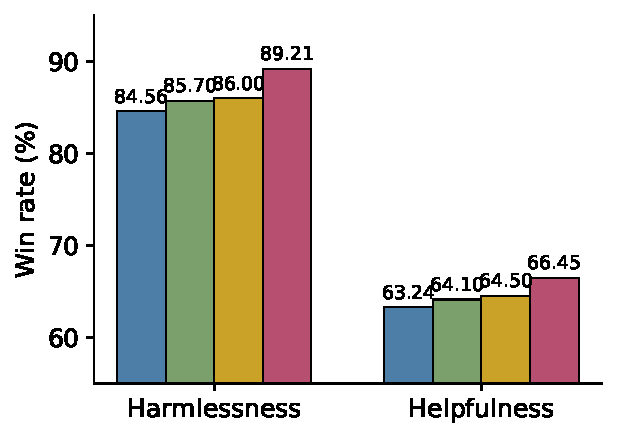
\includegraphics[width=\linewidth]{figures/ablation_winrate_combined.pdf}
        \vspace{0.3em}
        \scriptsize\textbf{(a) Qwen-2 0.5B}
    \end{minipage}\hfill
    \begin{minipage}[t]{0.48\linewidth}
        \centering
        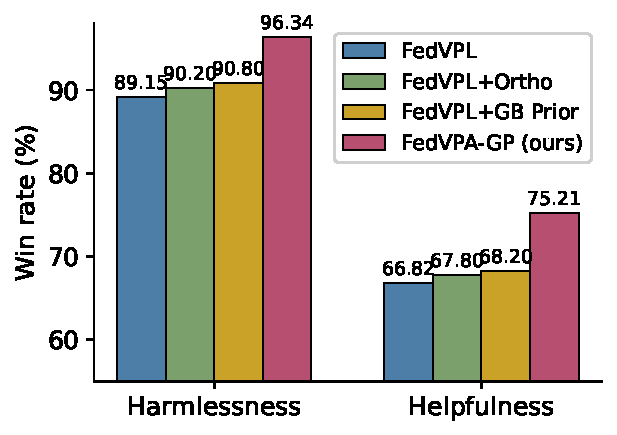
\includegraphics[width=\linewidth]{figures/ablation_winrate_combined_gemma.pdf}
        \vspace{0.3em}
        \scriptsize\textbf{(b) Gemma-2B}
    \end{minipage}
    \caption{Ablation study: helpfulness and harmlessness win rate (\%). (a) Qwen-2 0.5B. (b) Gemma-2B. Methods: FedVPL, FedVPL+Ortho, FedVPL+GB Prior, FedVPA-GP.}
    \label{fig:ablation}
\end{figure*}
 from main.tex.
% Paths assume main.tex is in repo root; else set \graphicspath{{docs/}}.
%
% Optional: \usepackage{subcaption} lets you use \subcaption{(a) Qwen-2 0.5B} etc.
% Below uses a single caption and (a)/(b) in text for maximum compatibility.

\begin{figure*}[t]
    \centering
    \begin{minipage}[t]{0.48\linewidth}
        \centering
        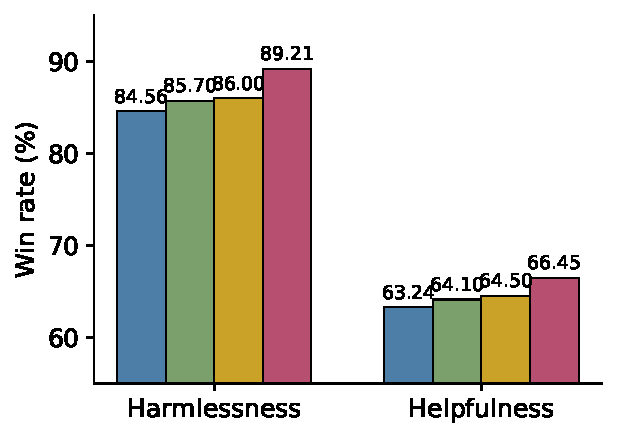
\includegraphics[width=\linewidth]{figures/ablation_winrate_combined.pdf}
        \vspace{0.3em}
        \scriptsize\textbf{(a) Qwen-2 0.5B}
    \end{minipage}\hfill
    \begin{minipage}[t]{0.48\linewidth}
        \centering
        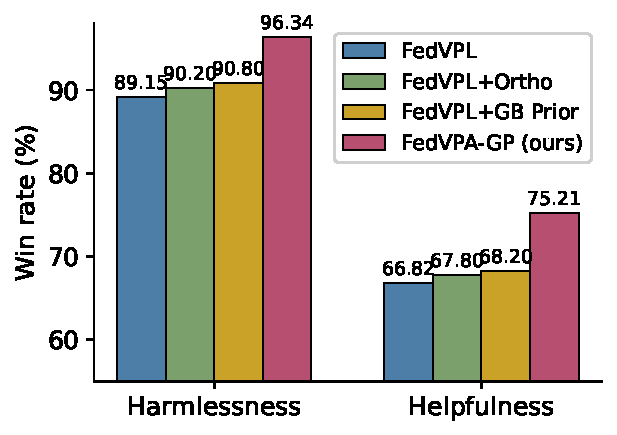
\includegraphics[width=\linewidth]{figures/ablation_winrate_combined_gemma.pdf}
        \vspace{0.3em}
        \scriptsize\textbf{(b) Gemma-2B}
    \end{minipage}
    \caption{Ablation study: helpfulness and harmlessness win rate (\%). (a) Qwen-2 0.5B. (b) Gemma-2B. Methods: FedVPL, FedVPL+Ortho, FedVPL+GB Prior, FedVPA-GP.}
    \label{fig:ablation}
\end{figure*}
 or % Ablation study: Qwen and Gemma win rate, two figures side by side.
% Usage: % Ablation study: Qwen and Gemma win rate, two figures side by side.
% Usage: \input{docs/ablation_figure} or \input{ablation_figure} from main.tex.
% Paths assume main.tex is in repo root; else set \graphicspath{{docs/}}.
%
% Optional: \usepackage{subcaption} lets you use \subcaption{(a) Qwen-2 0.5B} etc.
% Below uses a single caption and (a)/(b) in text for maximum compatibility.

\begin{figure*}[t]
    \centering
    \begin{minipage}[t]{0.48\linewidth}
        \centering
        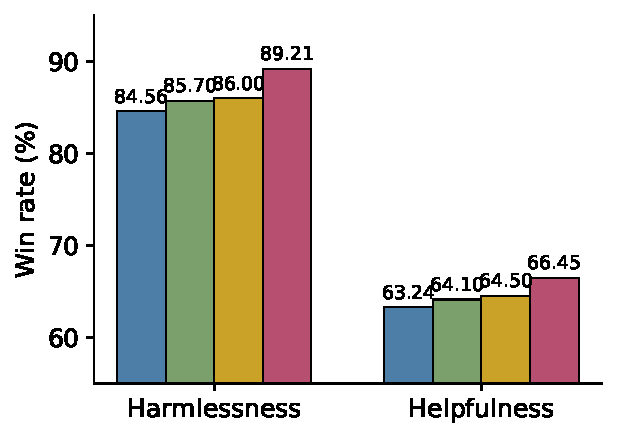
\includegraphics[width=\linewidth]{figures/ablation_winrate_combined.pdf}
        \vspace{0.3em}
        \scriptsize\textbf{(a) Qwen-2 0.5B}
    \end{minipage}\hfill
    \begin{minipage}[t]{0.48\linewidth}
        \centering
        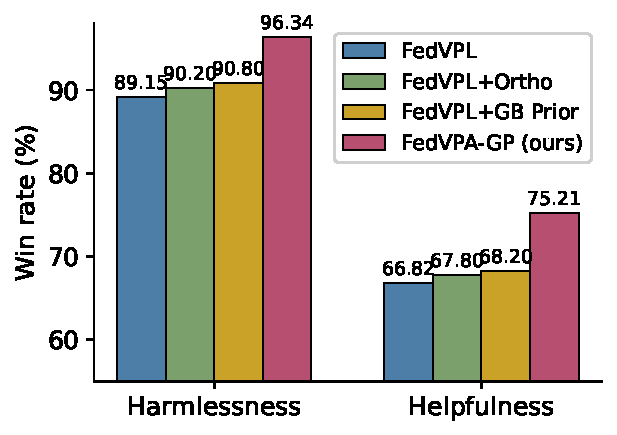
\includegraphics[width=\linewidth]{figures/ablation_winrate_combined_gemma.pdf}
        \vspace{0.3em}
        \scriptsize\textbf{(b) Gemma-2B}
    \end{minipage}
    \caption{Ablation study: helpfulness and harmlessness win rate (\%). (a) Qwen-2 0.5B. (b) Gemma-2B. Methods: FedVPL, FedVPL+Ortho, FedVPL+GB Prior, FedVPA-GP.}
    \label{fig:ablation}
\end{figure*}
 or % Ablation study: Qwen and Gemma win rate, two figures side by side.
% Usage: \input{docs/ablation_figure} or \input{ablation_figure} from main.tex.
% Paths assume main.tex is in repo root; else set \graphicspath{{docs/}}.
%
% Optional: \usepackage{subcaption} lets you use \subcaption{(a) Qwen-2 0.5B} etc.
% Below uses a single caption and (a)/(b) in text for maximum compatibility.

\begin{figure*}[t]
    \centering
    \begin{minipage}[t]{0.48\linewidth}
        \centering
        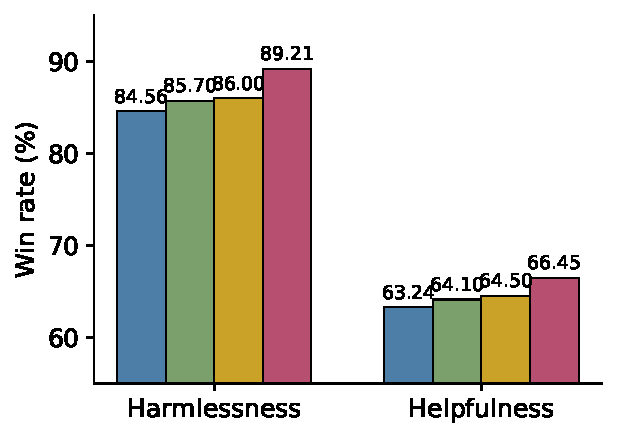
\includegraphics[width=\linewidth]{figures/ablation_winrate_combined.pdf}
        \vspace{0.3em}
        \scriptsize\textbf{(a) Qwen-2 0.5B}
    \end{minipage}\hfill
    \begin{minipage}[t]{0.48\linewidth}
        \centering
        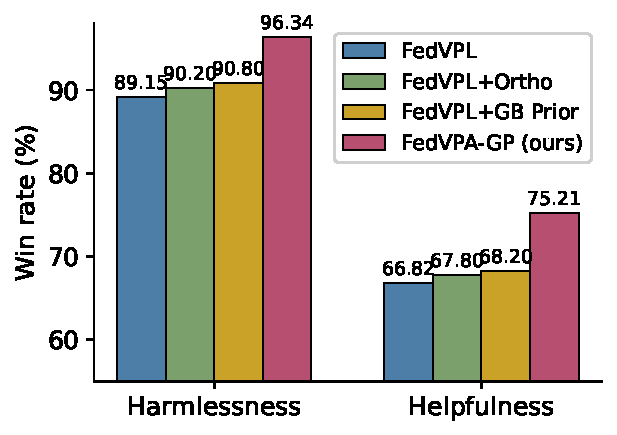
\includegraphics[width=\linewidth]{figures/ablation_winrate_combined_gemma.pdf}
        \vspace{0.3em}
        \scriptsize\textbf{(b) Gemma-2B}
    \end{minipage}
    \caption{Ablation study: helpfulness and harmlessness win rate (\%). (a) Qwen-2 0.5B. (b) Gemma-2B. Methods: FedVPL, FedVPL+Ortho, FedVPL+GB Prior, FedVPA-GP.}
    \label{fig:ablation}
\end{figure*}
 from main.tex.
% Paths assume main.tex is in repo root; else set \graphicspath{{docs/}}.
%
% Optional: \usepackage{subcaption} lets you use \subcaption{(a) Qwen-2 0.5B} etc.
% Below uses a single caption and (a)/(b) in text for maximum compatibility.

\begin{figure*}[t]
    \centering
    \begin{minipage}[t]{0.48\linewidth}
        \centering
        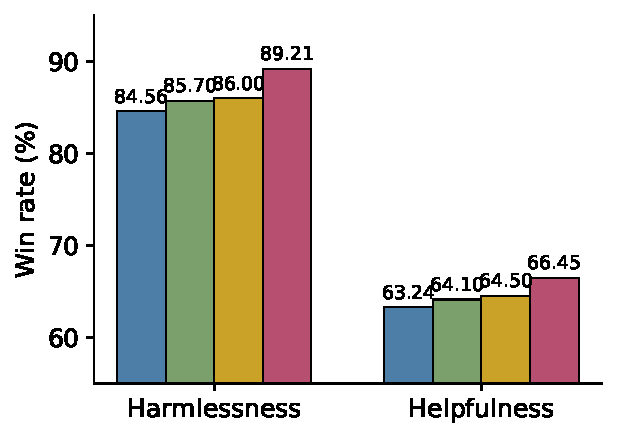
\includegraphics[width=\linewidth]{figures/ablation_winrate_combined.pdf}
        \vspace{0.3em}
        \scriptsize\textbf{(a) Qwen-2 0.5B}
    \end{minipage}\hfill
    \begin{minipage}[t]{0.48\linewidth}
        \centering
        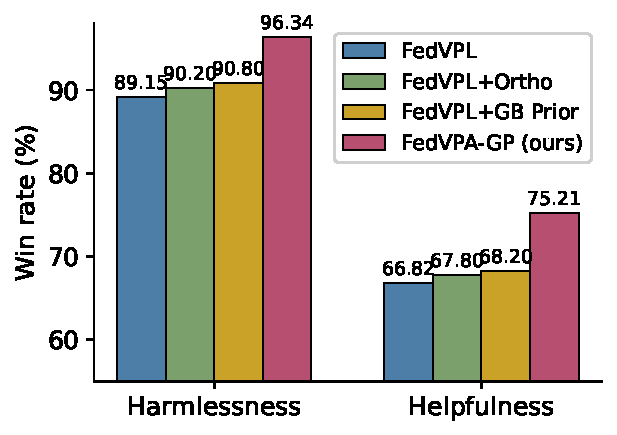
\includegraphics[width=\linewidth]{figures/ablation_winrate_combined_gemma.pdf}
        \vspace{0.3em}
        \scriptsize\textbf{(b) Gemma-2B}
    \end{minipage}
    \caption{Ablation study: helpfulness and harmlessness win rate (\%). (a) Qwen-2 0.5B. (b) Gemma-2B. Methods: FedVPL, FedVPL+Ortho, FedVPL+GB Prior, FedVPA-GP.}
    \label{fig:ablation}
\end{figure*}
 from main.tex.
% Paths assume main.tex is in repo root; else set \graphicspath{{docs/}}.
%
% Optional: \usepackage{subcaption} lets you use \subcaption{(a) Qwen-2 0.5B} etc.
% Below uses a single caption and (a)/(b) in text for maximum compatibility.

\begin{figure*}[t]
    \centering
    \begin{minipage}[t]{0.48\linewidth}
        \centering
        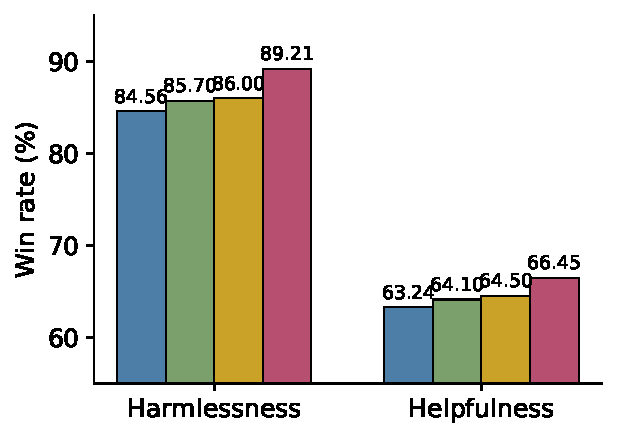
\includegraphics[width=\linewidth]{figures/ablation_winrate_combined.pdf}
        \vspace{0.3em}
        \scriptsize\textbf{(a) Qwen-2 0.5B}
    \end{minipage}\hfill
    \begin{minipage}[t]{0.48\linewidth}
        \centering
        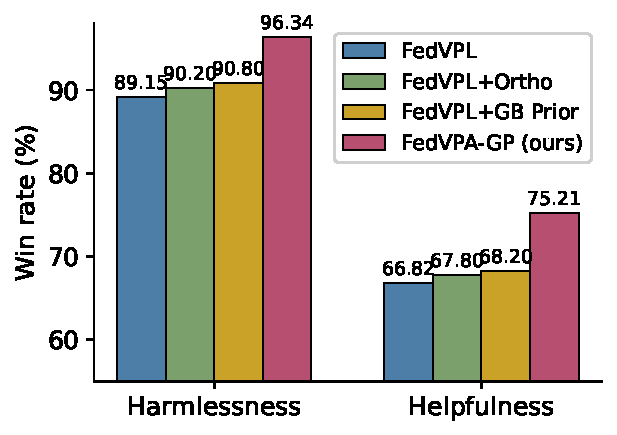
\includegraphics[width=\linewidth]{figures/ablation_winrate_combined_gemma.pdf}
        \vspace{0.3em}
        \scriptsize\textbf{(b) Gemma-2B}
    \end{minipage}
    \caption{Ablation study: helpfulness and harmlessness win rate (\%). (a) Qwen-2 0.5B. (b) Gemma-2B. Methods: FedVPL, FedVPL+Ortho, FedVPL+GB Prior, FedVPA-GP.}
    \label{fig:ablation}
\end{figure*}
 from main.tex.
% Paths assume main.tex is in repo root; else set \graphicspath{{docs/}}.
%
% Optional: \usepackage{subcaption} lets you use \subcaption{(a) Qwen-2 0.5B} etc.
% Below uses a single caption and (a)/(b) in text for maximum compatibility.

\begin{figure*}[t]
    \centering
    \begin{minipage}[t]{0.48\linewidth}
        \centering
        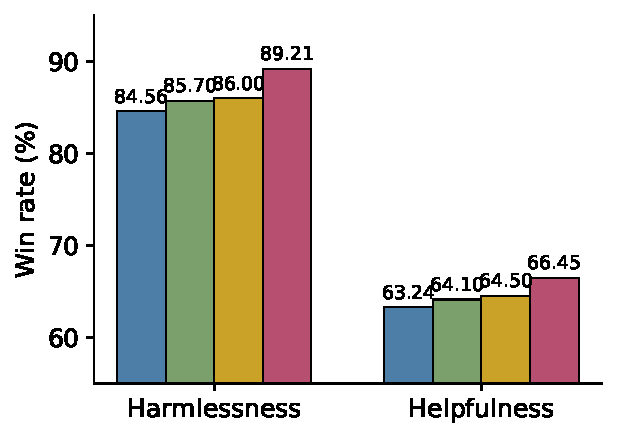
\includegraphics[width=\linewidth]{figures/ablation_winrate_combined.pdf}
        \vspace{0.3em}
        \scriptsize\textbf{(a) Qwen-2 0.5B}
    \end{minipage}\hfill
    \begin{minipage}[t]{0.48\linewidth}
        \centering
        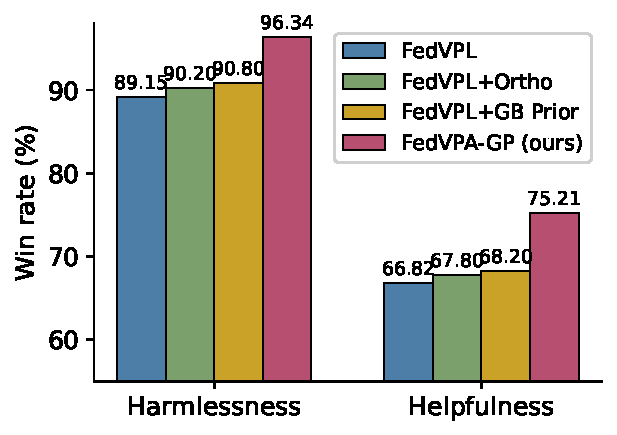
\includegraphics[width=\linewidth]{figures/ablation_winrate_combined_gemma.pdf}
        \vspace{0.3em}
        \scriptsize\textbf{(b) Gemma-2B}
    \end{minipage}
    \caption{Ablation study: helpfulness and harmlessness win rate (\%). (a) Qwen-2 0.5B. (b) Gemma-2B. Methods: FedVPL, FedVPL+Ortho, FedVPL+GB Prior, FedVPA-GP.}
    \label{fig:ablation}
\end{figure*}
